\section{Background}

\lettrine[lines=2]{\color{color2}T}{}he number of cases of SARS-CoV-2, responsible for the coronavirus disease 2019 (COVID-19), rose at an exponential rate and rapidly reached the status of a pandemic. In a cohort from China, the COVID-19 was associated with severe disease requiring intensive care in approximately 5\% of cases and the overall fatality rate was 2.3\%.The death rate for all infected patients may be in the range of 0.5\% to 5.6\% \cite{wu_characteristics_2020,baud_real_2020}. Among patients requiring hospitalization, the proportion of case-fatalities is between 5\% and 15\%. However, in patients who become critically ill, it ranges from 22\% to 62\% \cite{yang_clinical_2020,wang_clinical_2020}.
From ICU to the recovery period, the interventions of physiotherapists are essential to prevent potential acquired muscle weakness and to improve the functional recovery of patients. The objective of this article is to recall the main functional consequences of hospitalization and to synthesize the possible actions (Figure 1). A section is also devoted to post-hospital care.

\section{Factors associated with admission to intensive care} 
According to the latest available data, patients who require intensive care are older than patients who do not require intensive care (median age, 66[57-78] years vs 51[37-62] years), and 72.2\% have underlying comorbidities, commonly diabetes, respiratory and cardiac disease \cite{wu_characteristics_2020,wang_clinical_2020}. In a cohort study \cite{zhou_clinical_2020}, death was associated with older age, a higher Sequential Organ Failure Assessment (SOFA) score,  and d-dimer levels above 1·0 $\mu$g/L on admission. In this study, the median duration of viral shedding was 20 [17·0–24·0] days in survivors, but continued until death in fatal cases \cite{zhou_clinical_2020}. The most common symptoms on hospital admission were fever (94\%) and cough (79\%), followed by sputum production (23\%) and fatigue (23\%), which is concordant with the study by Yang et al. published early on \cite{yang_clinical_2020}. 

Given the severe acute respiratory infection the disease causes, intensive care is a key component of the management. The median time between symptom onset and admission to the Intensive Care Unit (ICU) has been reported to be 9.5[7–12.5] days, suggesting a gradual deterioration in the majority of cases \cite{yang_clinical_2020}. Two observational ICU studies showed that between 47\% and 71\% of patients admitted required invasive ventilation \cite{yang_clinical_2020,wang_clinical_2020}. Non-survivors were more likely to develop Acute Respiratory Distress Syndrome (ARDS) compared to survivors and were more likely to need mechanical ventilation \cite{yang_clinical_2020}. The most documented reason for requiring intensive care was for respiratory support, of which two-thirds of patients met the criteria for ARDS \cite{wang_clinical_2020}. In addition to respiratory failure, sepsis and heart failure are also reported to be common reasons for admission to intensive care and subsequent intubation \cite{zhou_clinical_2020,ruan_clinical_2020}.

\section{Hygiene procedures for COVID-19 transmission control}
\subsection{What is the risk of SARS-Cov-2 contamination for healthcare providers?}
The risk of nosocomial transmission of SARS-Cov-2 is high. One of the largest cohort reported revealed that a total of 1716 healthcare providers were contaminated out of 44672 confirmed cases of COVID-19. Around 15\% of these cases were classified as severe or critical and five deaths occurred \cite{wu_characteristics_2020}. All care providers (including physiotherapists) that manage individuals with COVID-19 should therefore be thorough with their own protective measures, especially when providing aerosol-generating procedures. Moreover, contaminated care providers may also contaminate other patients. Another important point to consider is that the mean incubation period for SARS-Cov-2 infection is 5.2 days, but it can be up to 14 days \cite{li_early_2020}. If available, physiotherapists should wear surgical masks when taking care of other patients, or at least the most vulnerable ones, even if they have no signs of COVID-19 infection. 

\subsection{What are the recommendations for the prevention and control of infection in care providers?}
One of the key components of infection prevention for the management of individuals with COVID-19 infection is staff education \cite{bouadma_severe_2020}. These measures involve taking precautions during all procedures that can generate aerosolization, droplets and contact. Personal Protective equipment (PPE) such as a surgical cap, a well-fitted high filtration mask (N95/FFP-2 masks), goggles or a face shield, a non-sterile, waterproof, long-sleeve gown and non-sterile gloves should be worn and at all times within the patient’s room. A complete alcohol-based hand rub should be performed before, during and after dressing and undressing. All this equipment should be removed in the antechamber and treated as infectious waste (except for face shields and goggles). Comprehensive guidelines for dressing and undressing procedures have been published \cite{bouadma_severe_2020}. Protective measures for non-aerosol generating procedures can be limited to surgical masks, the use of gloves, gowns and goggles \cite{long_effectiveness_2020}. No personal belongings should be brought into the patient’s room. Finally, all non-essential care procedures should be avoided to decrease the risk of viral transmission.

All therapists who are involved in aerosol-generating procedures and caring for patients on ventilatory support (Continuous positive airway pressure, Non-invasive Ventilation, High Flow Nasal Canula etc.) must use high levels of protection.

In the acute phase of a COVID-19 infection, caregivers should only enter the patient’s room if their presence is essential, and they should be equipped with the appropriate level of PPE \cite{wang2020challenges}. Aerosol’s procedures should be applied with an awareness of the potential risks of contamination, and the aim of each intervention should be determined before entering the room (\textbf{Figure 1}). The Surviving Sepsis Campaign guidelines on the management of critically ill patients with COVID-19 suggested using a surgical/medical mask rather than a high filtration mask in addition to contact and eye protection during non-aerosol-generating procedures such as the prevention or treatment of complications relating to bed rest. This recommendation is applicable for both non-ventilated patients and those under invasive mechanical ventilation (closed circuit) \cite{alhazzani_surviving_2020}. 

\section{Clinical Management in the ICU and Outcomes}

The management of severe cases of COVID-19 is very close from the management of other types of viral pneumonia that cause respiratory failure. The principal feature of patients with severe disease is the development of ARDS that is  characterized by a serious deterioration in gas exchange driven by alveolar and interstitial infiltrates \cite{ashbaugh_acute_1967}. Therefore, evidence-based treatment guidelines for ARDS should be followed, including conservative fluid strategies, antibiotic-therapy for potential bacterial co-infection, lung protective ventilation and prone positioning \cite{fan_official_2017}.

\section{Physiotherapy for patients on invasive mechanical ventilation}
\subsection{What are the consequences of mechanical ventilation?}
Approximately 50\% of patients admitted to ICU develop ICU-acquired weakness, which may increase the duration of mechanical ventilation \cite{zorowitz_icuacquired_2016}. ICU-acquired weakness may also persist for up to 5 years after hospital discharge, with a significant loss of functional capacity \cite{herridge_functional_2011}. The main contributors to ICU-acquired weakness are inflammation, metabolic disorders, and muscle rest during sedation or neuromuscular blockers, particularly in patients with sepsis and prolonged invasive mechanical ventilation \cite{batt_mechanism_2017,batt_intensive_2013}. A high proportion of COVID-19 patients are on invasive ventilation (71\% of required mechanical ventilation in the cohort by Yang et al. \cite{yang_clinical_2020}). It is therefore to be expected that the vast majority of these patients will develop ICU-acquired weakness. In addition to physical weakness, stays in ICU often result in cognitive and psychological impairments, which are collectively named post intensive care syndrome (PICS). There is a large body of evidence showing that muscle weakness is an independent factor associated with a higher rate of long-term mortality and a decrease in functional capacity \cite{vanhorebeek2020icu,van_aerde_five-year_2020}. A similar association has been found for PICS syndrome \cite{smith_home_2020}.

\subsection{How should muscle function be assessed in patients with COVID-19?}
Overall strength can be measured using the Medical Research Council sum-score (MRC-SS). ICU-acquired weakness is characterized by symmetrical impairment in the left and right limbs that is most prominent in proximal muscles \cite{vanhorebeek2020icu}. A score below 48/60 on the MRC scale indicates significant muscle weakness and is associated with an increase in the risk of ICU and hospital death \cite{medrinal_icu_2020}.

As the diaphragm can be severely affected during controlled ventilation, the switch to spontaneous ventilation should be done as soon as possible \cite{schepens_diaphragm_2020}. In addition, switching to spontaneous ventilation is essential for accurate assessment of respiratory muscle function. Maximum inspiratory pressure (MIP) is a simple measure of all the inspiratory muscles together. This measurement is often available on ventilators: a value below 30 cmH2O is defined as indicative of respiratory muscle weakness and predictive of difficult weaning from mechanical ventilation \cite{medrinal_respiratory_2016}. MIP measurements can be repeated daily to monitor progress and are considered valid in patients who respond to simple orders. The assessment of voluntary muscle strength (MRC-SS and MIP) is limited to patients who are both awake and cooperative. in non-cooperative patients, ultrasound is a reliable, sensitive, and valid tool to assess diaphragm \cite{dube_ultrasound_2017,jung_diaphragmatic_2016,le_neindre_thoracic_2016} and quadriceps strength \cite{formenti_clinical_2019}. 

Once sedation has been stopped or after weaning from mechanical ventilation, it is important to assess the patient’s functional capacity in order to guide further physical rehabilitation. Scales such as the 5-meter walk test or the 5 times sit-to-stand test may be useful \cite{nordon-craft_intensive_2012,haley_linking_2011}.

\subsection{Could airways clearance techniques help the patients?}

In patients on mechanical ventilation, chest physiotherapy does not lead to further improvements in ventilatory function or gas exchange \cite{goncalves_effects_2016}, therefore it is of no interest for patients with COVID-19.

\subsection{How to preserve functional capacity in patients in ICU?}

Neuromuscular Electrical Stimulation (NMES) is a non-invasive and easy to perform technique that does not require prolonged exposure of the physiotherapist to the patient. Several systematic reviews have suggested that NMES preserves muscle strength, mass and architecture \cite{burke2016evaluation,wageck_application_2014,parry_electrical_2013}. However, the results of the studies included in those systematic reviews are not always clinically relevant and need to be considered with caution\cite{zayed_effects_2020}. 

Early rehabilitation including passive mobilization exercises do not decrease the duration of hospitalization and mechanical ventilation in patients with acute respiratory failure \cite{morris_standardized_2016}. Interestingly, Griffiths et al. showed a modest benefit of passive mobilization on muscle trophicity when it was performed for three hours at a time, three times a day \cite{griffiths1995effect}, which is not feasible in clinical practice. Thus, in view of the absence of benefits described in the literature, passive range of motion exercises are not a priority intervention for patients on mechanical ventilation and should not be performed \cite{medrinal_comparison_2018}. 

A recent study showed that a comprehensive rehabilitation program including the addition of an in-bed cycle ergometer with quadriceps electrostimulation did not improve muscle strength more than standard rehabilitation alone with patients exercising out of bed \cite{fossat_effect_2018}. These results suggest that when patients can perform exercise out of bed, the use of an in-bed cycle-ergometer does not provide any additional benefit. However, in-bed cycle-ergometry could be considered for patients who cannot perform exercise out of bed because it may provide some benefit above no exercise. Functional electrical stimulation cycling could also be considered, because it provides more intense exercise than in-bed cycle-ergometry alone \cite{burtin_early_2009}.

In view of the lack of effectiveness of in-bed techniques, it is important to get the patient out of bed as soon as possible. A comprehensive physiotherapy program with out-of-bed exercises can increase muscle strength and recovery of functional capacity and reduce ICU delirium \cite{schweickert_early_2009}. Active exercises can be initiated once sedation has been stopped and when the patient can respond to simple orders. Patients who tolerate this can be actively positioned using different types of supportive devices (stretcher chairs, standing frames etc.). Passive verticalization on a tilt table does not affect muscle strength \cite{sarfati_efficacy_2018} and active verticalization should mostly be considered. Several studies have shown no benefits of intensive early rehabilitation  over standard rehabilitation including exercise out of bed \cite{moss_randomized_2016,wright_intensive_2018}. Therefore, in the context of COVID-19, intensive early rehabilitation should not be carried out.

The reduction in gas exchange associated with lung infection can cause severe hypoxemia during rehabilitation sessions. In patients with unstable SpO2 levels it is advisable to adjust their oxygen intake in order to maintain an SpO2 of 94\% during the training sessions \cite{thomas_physiotherapy_2020}. In order to limit desaturation, in the cases where oxygen intake cannot be adjusted, exercise intensity can also be decreased \cite{hillegass2014supplemental}.

Finally, considering the risk of transmission and the evidences, inspiratory muscles training using valve does not seem appropriate \cite{vorona_inspiratory_2018,elkins_inspiratory_2015}. In case of inspiratory muscle weakness, we recommend establishing a protocol in order to gradually decrease the levels of ventilatory support and monitor the evolution of inspiratory muscle strength.

\section{Physiotherapy for non-ventilated patients}
In view of the exceptional nature of the current health situation, a dedicated physiotherapist should be in charge of patients with COVID-19 whenever possible. If this is not possible, isolation procedures should be followed and physiotherapists in contact with patients with COVID-19 should not also treat vulnerable, non-infected patients. A meticulous organization of the care schedule and staff must be put in place to minimize the risk of transmission. Finally, the potential benefits of any intervention must constantly be weighed against any possible risk of cross-contamination. In patients who are less severely affected physiotherapists can limit their interventions to the provision of advice and instructions regarding exercises that the patient can perform independently (eg. standing up regularly, walking in the room every hour, use of elastic bands for strengthening; depending on the patient's tolerance and ability). Patients should be encouraged to sit out of bed as much as possible and to carry out their own activities of daily living \cite{thomas_physiotherapy_2020}.

\subsection{Are airway clearance techniques useful?}

Two published cohort studies reported that between 20 and 30\% of patients with COVID-19 produce sputum \cite{zhou_clinical_2020,guan_clinical_2020}. Nevertheless, it is noteworthy to mention that if the patient has an effective cough and does not retain secretions, the literature does not support the use of airways clearance techniques \cite{strickland_aarc_2013}: chest physiotherapy is not recommended as routine treatment for pneumonia in adults \cite{yang_chest_2013}. In addition, airway clearance techniques can tremendously increase the risk of contamination because of droplet dispersion in the environment. This is also the case for instrumental techniques (incentive spirometry, positive expiratory pressure masks, etc.) that can cause aerosolization and are therefore not advised \cite{simonds_evaluation_2010}. However, chest physiotherapy may be indicated for patients with underlying secretion clearing issues (such as bronchiectasis or cystic fibrosis) \cite{imam_non-cf_2020}.


\begin{figure}
\centering
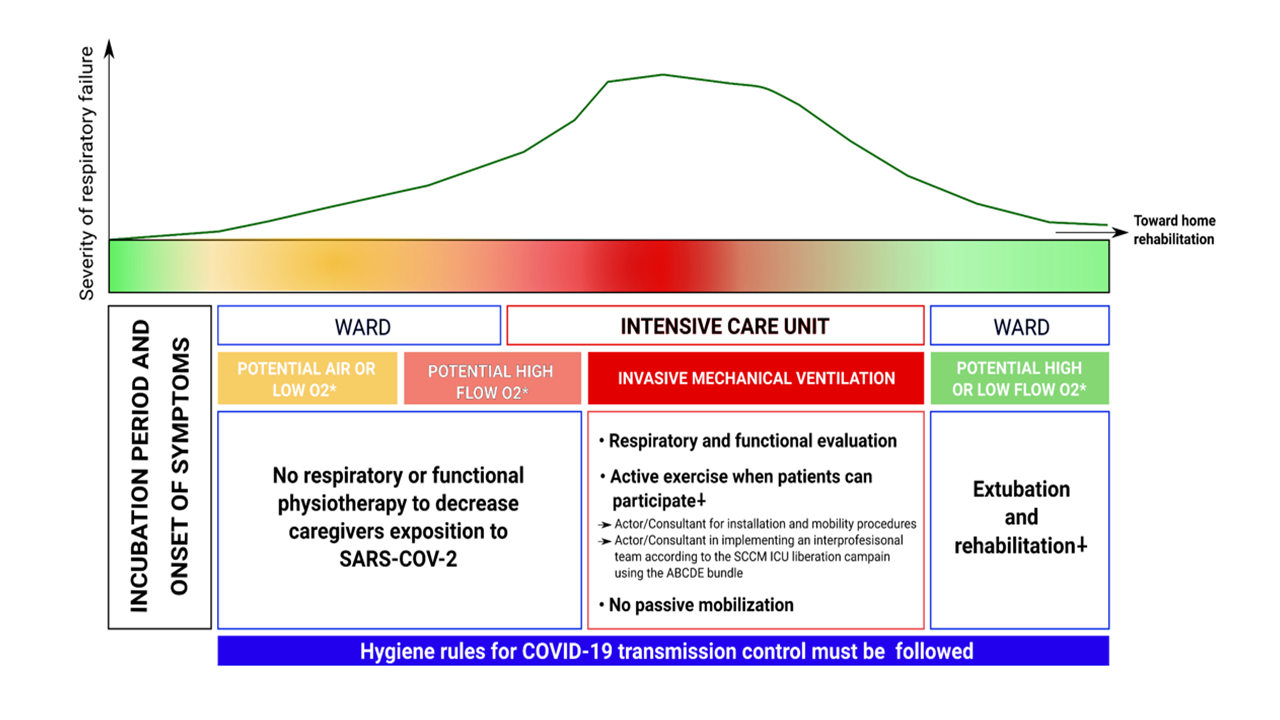
\includegraphics[width=\linewidth]{review/figure-1.png}
\caption{Clinical course and outcomes in critical care patients and management strategies for physiotherapists. Based on data from Wang et al.,Yang et al., Wu et al and Bouadma et al. \cite{wu_characteristics_2020,wang_clinical_2020,alhazzani_surviving_2020,medrinal_icu_2020}. \textit{aerosol-generating procedure; non aerosol-generating procedure". ABCDE: Awakening and Breathing Coordination, Delirium, and Early exercise/mobility; NEMS: Neuromuscular Electrical Stimulation; O2: oxygen} 
}%
\end{figure}

\section{Physiotherapy following discharge from intensive care }
Evidence regarding the potential long-term consequences of viral infections causing acute severe respiratory diseases is scarce. Data from the influenza A epidemics showed that survivors had substantial alterations in their lung function up to 2 years after being discharged from hospital \cite{chen_long_2017,liu_pulmonary_2015}. In addition to impaired lung function, exercise capacity is markedly reduced in survivors \cite{ong_pulmonary_2004,hui_impact_2005}. In the COVID-19 epidemic, a large number of patients admitted to the ICU develop ARDS \cite{wang_clinical_2020}. This condition is strongly correlated with a decrease in long-term functional capacity \cite{herridge_one-year_2003}, in particular muscle strength and walking distance \cite{bein_long-term_2018}. Ong et al. showed that 41\% of subjects had a loss of maximum aerobic capacity compared to normal values 3 months after hospital discharge \cite{ong_pulmonary_2004}. Exercise capacity is an important determinant of quality of life. Data from 110 SARS survivors showed they had a significantly reduced quality of life compared to the general population \cite{hui_impact_2005}. Finally, the long-term consequences of ARDS on mental health should not be overlooked. Depression and anxiety are also very common in survivors of ARDS, with a prevalence above 26\% and 28\% respectively \cite{bein_long-term_2018}. 

\subsection{How to continue physiotherapy after discharge?}
Patients who have been ventilated for more than seven days and who have a significant loss of functional capacity are likely to respond the best to an inpatient or day-care rehabilitation program. This group of patients is at higher risk of hospital readmission should be closely monitored \cite{herridge_recover_2016}. Those patients, and their rehabilitation needs, can be identified by physiotherapists through simple functional tests such as the sit to stand test (30 seconds or one minute), the time up and go test (TUG) or the physical function in ICU test (PFIT test). In order to prevent cross-transmission of the virus, it is not useful to provide  supervised rehabilitation to patients who are independent, have no muscle weakness or who have a low risk of deconditioning \cite{noauthor_covid-19_2020}. In this case tele-rehabilitation could be discussed.

For patients who do not have access to a rehabilitation center, treatment at home or in an out-patient physiotherapy practice should be considered. The provision of a booklet containing a six-week program of home exercises has been shown to optimize functional recovery \cite{jones_rehabilitation_2003}. The exercises should be simple with minimal need for equipment (e.g. standing up from a chair, climbing stairs, walking 30 minutes a day, strengthening exercises using bottles of water etc.). The intensity of physical activity should be low (3 on the modified Borg scale) for the first 6 to 8 weeks after discharge from hospital \cite{noauthor_covid-19_2020}. The proportion of patients with COVID-19 and severe residual hypoxemia during exercise is currently unknown. Physiotherapists should monitor SpO2 during exercise to measure the severity of hypoxemia. If the patient uses oxygen, titration is recommended in order to maintain 90\%SpO2 \cite{hillegass2014supplemental}. For patients who are not on oxygen, supplementation should be discussed with their physician and the intensity of the exercise should be reduced. 

To increase patient adherence to a home exercise program, the patient can be instructed to keep a log-book of daily activities and to identify any barriers that prevent him/her from carrying out any activities. Simple tools such as a pedometer can be useful to motivate patients. A weekly follow-up telephone call or a home visit  may be necessary to supervise the exercise program, answer the patient's questions and provide motivational coaching \cite{holland_home-based_2017}. Tele-rehabilitation can also be useful \cite{bonnevie2019people} and could be particularly appropriate in the context of the COVID-19 epidemic.

\section{Conclusion}
The COVID-19 pandemic is one of the largest that the world has faced in the last fifty years, resulting in a high number of hospitalizations and saturating intensive care units. In this context, physiotherapists have an important role to play in helping patients return to their highest level of function, in the ICU or following discharge from the hospital. 
Finally, in view of the very high proportion of patients who are likely to have persistent loss of functional capacity following discharge, clinical research should aim to rapidly evaluate new management strategies and tools such as tele-rehabilitation and unsupervised rehabilitation in order to help patients to regain physical and cognitive function.
